\documentclass[a4paper, 11pt, twocolumn]{article}
\usepackage[utf8]{inputenc}
\usepackage{graphicx}
\usepackage[T1]{fontenc}
\usepackage[ngerman]{babel}
\usepackage{graphicx} 
\usepackage{layout} 
\usepackage{geometry}
\usepackage{subfigure}
\usepackage{fancyhdr}
\usepackage{expdlist}
\usepackage{makeidx}
\usepackage{tabularx}
\usepackage{multirow}
\usepackage{amsmath,amssymb,amstext}

\fancyfoot[C]{\thepage}%  Spezielle Fusszeile
\begin{document}

\title{\textbf{Tracking von Gesichtern in belebten Umgebungen mit Hilfe eines Partikelfilters}}
\author{ \textit{Kai Wolf} \\ Kai.B.Wolf@student.hs-rm.de\vspace{0.8cm}\\Hochschule RheinMain\\University of Applied Sciences\\Wiesbaden Rüsselsheim Geisenheim}
\date{\today\\[5mm]
\begin{center}
\textbf{Zusammenfassung}\\[2mm]
\begin{minipage}{0.9\textwidth}
Dieses Projekt ist im Rahmen der Vertiefungsveranstaltung Machine Learning im Masterstudiengang Informatik an der Hochschule RheinMain entstanden. Die Veranstaltung fand im Sommersemester 2012 statt und wurde von Prof. Dr. Schwanecke betreut. Die vorliegende Arbeit behandelt das automatisierte Tracking von Personen anhand des Gesichts in belebten Umgebungen. Dabei werden klassifizierte Personen mit Hilfe eines Partikelfilters über mehrere Frames hinweg verfolgt. Der Quelltext zu dieser Arbeit basiert weitestgehend auf der Veröffentlichung aus dem Jahr 2009~\cite{aliMultipleHuman}.
\end{minipage}
\end{center}
} 
\maketitle

\section{Einleitung} % (fold)
\label{sec:einleitung}
Das automatisierte Tracking von Personen in einem Videobild ist eine anspruchsvolle Aufgabe aus dem Bereich Machine Learning. Dabei müssen gleich mehrere Problemstellungen gelöst werden: Erfolgreiche Erkennung von gesuchten Objekten im Videobild, Verfolgung der zuvor entdeckten Objekte über mehrere Frames hinweg und schließlich die Anpassung der Verfolgung unter Einbeziehung des Verhaltens des Objekts~\cite{Yilmaz2006}. 
Das Gesicht einer Person ist im Allgemeinen ein stabiles Feature für die Wiedererkennung~\cite{ViolaRobustObject2001}. Dennoch können bei der Detektion gleich mehrere Probleme auftreten: 
Zum einen kann die Erkennung von Gesichtern aufgrund von Schatten oder starken Reflektionen beeinträchtigt werden, zum anderen können Gesichter gerade in belebten Umgebungen wie Straßen oder Fussgängerzonen durch andere Menschen oder Gebäude teilweise oder ganz verdeckt werden~\cite{aliMultipleHuman}. 
Die vorliegende Arbeit verwendet zur Lösung der aufgezählten Probleme einen robusten Viola-Jones-Klassifikator zum Erkennen von Gesichtern und einen Partikelfilter für das Tracking über mehrere Frames. Dabei wird für jedes klassifizierte Gesicht ein Bewegungspfad initialisiert, der die Bewegung einer Person anhand ihres Gesichts über mehrere Frames hinweg verfolgt. Durch das in~\cite{aliMultipleHuman} beschriebene \emph{confirmation-by-classification}-Verfahren wird für jeden Frame erneut der Gesichtsklassifikator benutzt, der für jedes klassifizierte Gesicht rund um die zuletzt gemessene Position erneut nach Gesichtern sucht und dem dazugehörigen Bewegungspfad zuordnet. 

% section einleitung (end)

\section{Bisherige Arbeiten} % (fold)
\label{sec:bisherige_arbeiten}

Für das automatisierte Tracking von Personen in einem Videobild existieren verschiedene Ansätze, die das Tracking von Personen über ein Bewegungsmodel realisieren. In der Arbeit von~\cite{zhaoSegmentationTracking} wird die Bewegung einer Person anhand des starr bleibenden Hintergrunds detektiert. In der Veröffentlichung von~\cite{Zhao2004} werden Personen anhand ihrer Körperform identifiziert und die Tatsache genutzt, dass diese (meist) auf einer Ebene durch das Videobild laufen. Eine etwas ältere Arbeit aus dem Jahr 2001 identifiziert Objekte anhand ihrer Features, die zusammengenommen, in nachfolgenden Frames wiedergefunden werden können~\cite{Veenman2001}.

Alle diese Verfahren funktionieren jedoch bei steigender Anzahl von Personen im Videobild nicht mehr richtig, da dadurch gesamte Szene in Bewegung gerät oder viele Personen im Bild durch andere Personen oder Gegenstände teilweise oder komplett verdeckt werden. Unter diesen Bedingungen stellt das Gesicht einer Person das einzige Feature dar, das in einem Videobild stabil wiedererkannt werden kann~\cite{aliMultipleHuman}.

% section bisherige_arbeiten (end)

\section{Statistische Filter} % (fold)
\label{sec:statistische_filter}

Die sog. Klasse der \emph{statistischen Filter} zeichnen sich durch drei Besonderheiten aus: Statistische Filter fassen Messwerte als Wahrscheinlichkeitsverteilungen auf. Gegenüber der traditionellen Statistik, in welcher die Wahrscheinlichkeit als Sicherheit bzw. Unsicherheit über des Eintreten eines Ereignisses eines Zufallsexperiments definiert ist, benötigen statistische Filter kein Zufallsexperiment als Grundlage. 
Des Weiteren werden immer bedingte Wahrscheinlichkeit der Form $P(B|A)$ betrachtet. Das bedeutet, es wird die Wahrscheinlichkeit geschätzt, wie plausibel es ist, dass Aussage B eintritt, unter der Voraussetzung, dass A eingetreten ist. Die Berechnung erfolgt mit Hilfe des \emph{Satz von Bayes}~\cite{PapulaFormelsammlung2001}:
\[
	P(B|A) = \frac{P(A \cap B)}{P(A)}
\]
Die dritte Besonderheit ist, dass unbekannte Parameter ebenfalls Zufallsvariablen sind. Das bedeutet insbesondere, dass diese nicht konstant sein müssen.
Einer der am häufigsten eingesetzten statistischen Filter ist die Klasse der sogenannten \emph{Kalman-Filter}~\cite{MarslandBook}.

% section statistische_filter (end)

\subsection{Kalman-Filter} % (fold)
\label{sub:kalman_filter}

Ein generelles Problem beim Tracking von Objekten ist, dass der aktuelle Ort von Objekten nicht direkt, sondern lediglich über Messungen zugänglich ist. In diesem Fall spricht man von sog. verborgenen Zuständen (engl. \emph{hidden states}). Solche Messungen sind aber grundsätzlich immer fehlerbehaftet. Das bedeutet, dass eine Messung nicht den wahren Ort wiedergibt. Man kann aber mit dem Messergebnis den aktuellen unbekannten Ort schätzen.

Das Kalman-Filter ist ein rekursiv arbeitender Filter, der für ein gegebenes System den nachfolgenden (diskreten) Systemzustand unter Berücksichtigung von normalverteilten Fehlern voraussagt. Dabei wird angenommen, dass die Veränderung des Systemzustands linear und a-priori bekannt ist~\cite{Welch1995}. Seien die Messwerte m durch Vektoren dargestellt. Dann sei $X_k$ der Zustand des Systems zum Zeitpunkt $t_k, X_k \in R^m$. Die einzelnen Systemzustände sind diskret, d.h. $t_k = t_0 + k \cdot \delta t$. Der aktuelle Systemzustand $X_k$ lässt sich mit Hilfe des vorangegangenen Zustands $X_{k-1}$ durch folgende lineare Gleichung modellieren:
\[
	X_k = F_{k-1} \cdot X_{k-1} + B_{k-1} \cdot u_{k-1} + w_{k-1}
\]
Dabei ist $F_{k-1}$ die Zustandsübergangsmatrix, $B_{k-1}$ die Dynamik der Störung (ebenfalls modelliert über eine Matrix), $u_{k-1}$ eine deterministische Störung und $w_{k-1}$ ein zufälliges Rauschen. Die einzelnen $w_i$ sind eine stochastische Größe, modelliert durch eine Normalverteilung mit dem Mittelwert 0 und der Kovarianzmatrix $Q_i$. Die einzelnen $\sum_{k=0}^k~X_k$ bilden einen stochastischen Prozess (eine sogenannte Markov-Kette). Dabei hängt das aktuelle $X_k$ nur von seinem Vorgänger $X_{k-1}$ ab (Markov-Modell erster Ordnung).

Die $X_k$ sind nicht direkt bekannt, sondern werden, wie zuvor erwähnt, durch eine (fehlerbehaftete) Messung ermittelt. Sei $Z_k$ die Messung des Systemzustands zum Zeitpunkt $t_k, Z_k \in R^m$. Der Zusammenhang zwischen dem Systemzustand und der Messung wird durch die lineare Gleichung:
\[
	Z_k = H_k \cdot X_{k-1} + v_k
\]

modelliert. Dabei ist $H_k$ die Beobachtungsmatrix und die $v_k$ eine stochastische Größe modelliert durch eine Normalverteilung mit Mittelwert 0 und der Kovarianzmatrix $R_i$. Die $v_i$ sind dabei unabhängig von den $w_i$ (Hidden-Markov-Model~\cite{MarslandBook}). 
\begin{figure}[htpb]
	\centering
	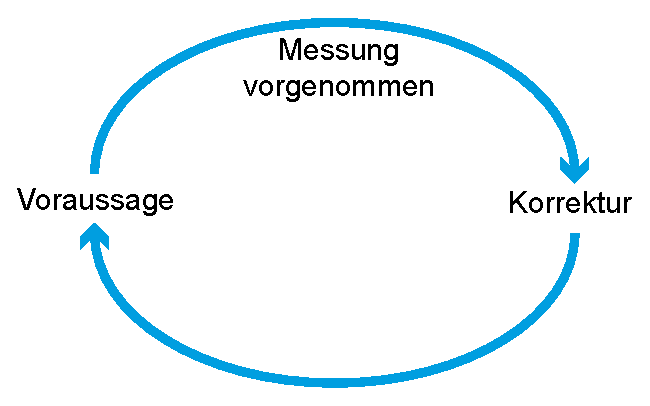
\includegraphics[width=0.5\textwidth]{kalman.eps}
	\caption{Prinzipielle Vorgehensweise eines Kalman-Filters}
	\label{fig:kalman}
\end{figure}
Für die Zufallsvariable $Z_k$ nimmt man konkrete Messungen vor, mit denen sich der Systemzustand $\widehat{X}_k$ zum Zeitpunkt $t_k, \widehat{X}_k \in R^m$ schätzen lässt. Das $\widehat{X}_k$ ist dabei eine normalverteilte Zufallsvariable mit dem Mittelwert $\widehat{m}_k$ und der Kovarianz $\widehat{P}_k$.
Die beiden Variablen werden initial mit $\widehat{m}_0 = 0$ und $\widehat{P}_0$ mit der Einheitsmatrix initialisiert. 

% subsection kalman_filter (end)

\subsection{Partikelfilter} % (fold)
\label{sub:partikelfilter}

Das Kalman-Filter liefert in der Regel gute Ergebnisse unter Annahme von normalverteilten Fehlern (Störgrößen) und einem linearen Prozessmodell~\cite{MarslandBook}. Sobald diese Bedingungen nicht mehr vorliegen, versagt das Kalman-Filter, da die Fehlererwartung nicht mehr gauss-verteilt ist.

Daher verfolgen Partikelfilter den Ansatz die aktuelle unbekannte Wahrscheinlichkeitsverteilung zu schätzen, um anschließend eine Aussage über den wahrscheinlichsten Systemzustand (des dynamischen Systems) zu treffen\cite{Doucet2009}. Hierfür wird ein Schwarm sogenannter Partikel erzeugt. Jedes Partikel besteht aus einem Gewicht und einem Punkt. Der Schwarm repräsentiert als Ganzes die Wahrscheinlichkeitsdichte in einem Anfangszustand, d.h. jedes Partikel repräsentiert einen möglichen Zustand. Anschließend wird für jeden Folgezustand des Systems anhand eines bestimmten Bewegungsmodells jedes Partikel neu platziert und das Gewicht anhand eines Erscheinungsmodells neu berechnet. Danach erfolgt mit Hilfe der neu berechneten Gewichte ein sog. \emph{Resampling} aller Partikel.

....

% subsection partikelfilter (end)

\section{Gesichtserkennung und Tracking} % (fold)
\label{sec:gesichtserkennung_und_tracking}

% Motion Model
% Appearance Model
% confirmation-by-classification

% section gesichtserkennung_und_tracking (end)

\section{Implementierung} % (fold)
\label{sec:implementierung}

Der Quelltext zu dieser Arbeit entstand unter Vorlage der Originalarbeit (vgl.~\cite{aliMultipleHuman}). Für die Verarbeitung des Videos wurde die freie Programmbibliothek OpenCV in der Version 2.4 verwendet.
Für die Gesichtserkennung wurde ein bereits trainierter Viola-Jones Klassifikator eingesetzt.
Für das Training des Klassifikators wurden 4325 Gesichter aus Videos unterschiedlicher Orte ausgeschnitten und auf die Größe von 20x20 Pixel skaliert. Des Weiteren wurde 2200 Negativbilder benutzt, um den Klassifikator zu trainieren.

Zur Verfolgung der Personen im Video wird initial der erste Frame des Videos in der Klasse \textbf{adaboostDetect.cpp} in ein Graustufenbild umgewandelt und auf 90\% der ursprünglichen Größe herunterskaliert. Anschließend erfolgt ein Histogrammausgleich des Bilds. Mit Hilfe der Funktion \textbf{cvHaarDetectObjects} wird die max. Anzahl an Gesichtern im Bild erkannt. Falls ein erkanntes Gesicht innerhalb vorgegebener Parameter (Größe) liegt, werden die Rechteckkoordinaten rund um das Gesicht gespeichert.

Danach erfolgt die Initialisierung des Trackers in \textbf{tracker.cpp}. Für das Tracking wird der aktuelle Frame in das HSV-Farbschema konvertiert und der Partikelfilter mit einer vorgegebenen Anzahl von 20 Partikel pro Objekt initialisiert (\textbf{particleFilter.cpp}). Für jedes zuvor erkannte Gesicht wird ein Bewegungspfad initialisiert. Jeder Bewegungspfad erhält die ID des aktuellen Frames, in welchem er initialisiert wurde, sowie ein Startgewicht von 1, ein Histogramm der entsprechenden Region um das Gesicht und die Koordinaten des dazugehörigen Partikelzentrums.

Für die Verfolgung der Gesichter wird anschließend jeder weitere Frame zuerst in das HSV-Farbschema umgewandelt (innerhalb der Funktion \textbf{tracker::next()}) und danach für alle Bewegungspfade die Partikel und Gewichte aktualisiert. Anschließend erfolgt das Resampling des Partikelfilters. In jedem Frame wird nun erneut nach Gesichtern gesucht. Jedes erkannte Gesicht wird entweder dem dazugehörigen Bewegungspfad zugeordnet, sofern der Abstand zwischen erkanntem Gesicht im Bild und Bewegungspfad ein Maximum nicht überschreitet oder ein neuer Bewegungspfad initialisiert. Falls für bestimmte Bewegungspfade die dazugehörigen Gesichter nicht mehr erkannt wurden, wird das Gewicht für diesen Bewegungspfad um einen konstanten Wert (hier 0.5) erniedrigt. Falls das Gewicht eines Bewegungspfad kleiner -3 wird, dann wird dieser Bewegungspfad komplett aus dem Tracking genommen.

% section implementierung (end)

\section{Evaluation} % (fold)
\label{sec:evaluation}

Für die Evaluation wurde ein Video aus der Münchener Fussgängerzone\footnote{http://www.youtube.com/watch?v=TdFvJ5ye7J8} verwendet. Ein Beispielbild aus dem Video ist in Abbildung~\ref{fig:fussgaenger_muenchen} zu sehen.

\begin{figure}[tb]
	\begin{center}
		\includegraphics[width=0.5\textwidth]{fussgaenger1.png}
	\end{center}
	\caption{Beispielbild aus der Münchener Fussgängerzone}
	\label{fig:fussgaenger_muenchen}
\end{figure}
	
Das Video hat eine Auflösung von 480x272 Pixeln und eine Länge von insgesamt 29 Sekunden. Eine manuelle Auswertung ergab, dass sich insgesamt 48 verschiedene Personen durch das Bild bewegen. Während des Videos befinden sich maximal 16 Personen gleichzeitig im Videobild. 

\begin{figure}[htpb]
	\subfigure[Automatisches Tracking]{\includegraphics[width=0.5\textwidth]{maxAnzahlFussgaengerAuto.png}}\hfill
	\subfigure[Manuelle Auswertung]{\includegraphics[width=0.5\textwidth]{maxAnzahlFussgaengerHand.png}}
	\caption{Vergleich von automatischem Tracking und manueller Auswertung bei maximaler Anzahl an Personen im Videobild}
	\label{fig:maxanzahl_fussgaenger}
\end{figure}

Wie in Abbildung~\ref{fig:maxanzahl_fussgaenger} zu sehen, klassifiziert der verwendete Algorithmus zum belebtesten Zeitpunkt des Videos insgesamt 9 Objekte. Dabei sind lediglich 5 Objekte tatsächlich Gesichter von Personen, während die übrigen Klassifikationen Taschen sind. Eine manuelle Auswertung ergibt eine tatsächliche Anzahl von 16 Personen im Bild, wobei davon 6 Personen teilweise bzw. ganz verdeckt sind. Das ergibt eine Trefferquote von 31.25\%.

\begin{figure}[htpb]
	\begin{center}
		\includegraphics[width=0.5\textwidth]{maxAnzahlFussgaengerTotal.png}
	\end{center}
	\caption{Maximale Anzahl gleichzeitig getrackter Objekte}
	\label{fig:maxanzahl_total}
\end{figure}

Der Algorithmus trackte maximal 12 Objekte gleichzeitig, wovon 6 Objekte tatsächlich Gesichter gewesen sind.

% section evaluation (end)

\section{Zusammenfassung} % (fold)
\label{sec:zusammenfassung}

Das vollständige und automatisierte Tracking aller Personen in einem Videobild stellt immer noch eine große Herausforderung aus dem Bereich Machine Learning dar. Es zeigte sich, dass der verwendete Algorithmus unter idealen Bedingungen, d.h. Gesicht vollständig sichtbar und Abstand zur Kamera innerhalb der verwendeten Parameter, gute Ergebnisse liefert. Dabei stellte die Blickrichtung der Person, sofern diese nicht völlig abgewandt zur Kamera stand, keine Probleme dar. Die teilweise Verdeckung des Gesichts hingegen, zum Beispiel durch andere Personen, Gegenstände, Gebäude oder Hände verschlechterte die Erkennungsrate deutlich.

% section zusammenfassung (end)

\bibliographystyle{apalike}
\bibliography{/Users/kai/Documents/library}

\end{document}